\documentclass[conference]{IEEEtran}
\usepackage{cite}
\usepackage{graphicx}
\usepackage{booktabs}
\usepackage{url}
\usepackage{xurl}
\usepackage[T1]{fontenc}
\usepackage{mathptmx}
\begin{document}

\title{An Agent-Based Model of Red-Striped Soft Scale Insect Management on Sugarcane in Negros Island}

\author{\IEEEauthorblockN{Joanne Maryz Cabatingan and Zenith O. Arnejo}
\IEEEauthorblockA{Institute of Computer Science, University of the Philippines Los Ba\~{n}os\\
Laguna, Philippines}}

\maketitle

\begin{abstract}
The red-striped soft scale insect (RSSI), \emph{Pulvinaria tenuivalvata}, had affected 72,103 ha of sugarcane on Negros Island by 2 October 2026, 30.1\% of the area planted. The two provinces have taken different courses, one funding biological control and the other chemical spraying, yet the pest's effect on yield has not been measured in the Philippines. This study develops an agent-based model of RSSI management in GAMA. A stage-structured pest, built from Philippine laboratory biology, runs on the cane landscape of all of Negros at 1-ha resolution, starting from the 87 ha declared infested on 22 May 2025. Farmers treat at infestation levels taken from the provincial monitoring survey, and parameters without a source are swept. Four strategies are compared over three crop years: no control, chemical control whose efficacy may decline with repeated use, biological control with an entomopathogenic fungus, and a hybrid of the two. Every control strategy cut cumulative pest load by at least 82\% relative to no control. Chemical control matched or beat biological control only if its efficacy halved no faster than about every 80 applications per farm. The hybrid added nothing over biological control while fungal efficacy held, but it gave the lowest load when both agents lost efficacy quickly. The ranking held in 15 of 18 one-at-a-time sensitivity cases. At baseline the model spread more slowly than the SRA record. The results are relative comparisons under stated assumptions, not field predictions.
\end{abstract}

\begin{IEEEkeywords}
agent-based model, GAMA, pest management, red-striped soft scale insect, sugarcane, sensitivity analysis
\end{IEEEkeywords}

\section{Introduction}

Negros Island accounts for about 57\% of the Philippine sugarcane area \cite{PCAARRDnd}, and its crop has faced a new pest since 2025. RSSI is a sap-feeding soft scale that excretes honeydew, on which sooty mould grows and interferes with photosynthesis \cite{Guerrero2026}. Under Philippine laboratory conditions a female lays about 197 eggs, reproduces without mating, and lives about 63 days from egg to death \cite{Guerrero2026}. The insect was first observed in the country in Pampanga in June 2022 \cite{Navasero2023}. In Negros it was first noted in northern Negros Occidental in late March 2025 and was declared an infestation on 22 May 2025, when it had spread over 87 ha \cite{ManilaBulletin2025}. By 2 October 2026 the Sugar Regulatory Administration (SRA) had validated 72,103 ha of affected cane, 30.1\% of the 239,216 ha planted in crop year 2025--2026 \cite{SRA2026FOI}. Both provinces declared a state of calamity \cite{Masculino2025,Bayoran2026,Partlow2026}.

The response mixes chemical spraying, including by drone, with biological control \cite{ChiniMandi2026}. The provincial government of Negros Occidental declined to fund chemical spraying and chose biological control without banning chemicals \cite{Bayoran2026}, while Negros Oriental planned chemical spraying of all its cane fields \cite{Partlow2026}. Its task force applies the fungi \emph{Metarhizium} and \emph{Beauveria} and classifies farms by infestation level \cite{PGNO2026}. No model in the review below compares these strategies over repeated use. The effect of RSSI on cane yield has not been studied in the Philippines \cite{Guerrero2024}, and an RSSI researcher stated that no rate of spread between fields can be calculated (G.~A.~S. Burgonio, pers.\ comm., 21 Sep.\ 2026).

This study builds an agent-based model to compare no control, chemical, biological, and hybrid control under these gaps. Its contribution is a model of a sessile scale insect on a real cane landscape, with a farmer choice between control agents on top of a stage-structured pest, and an explicit record of which inputs are measured and which are assumed. The outputs are relative comparisons between strategies, not forecasts.

\section{Related Work}

A systematic review following PRISMA 2020 \cite{Page2021} searched Web of Science and Scopus with one string and retained 30 agent-based or individual-based models of insect pests and their management from 426 records. Five model sugarcane, all for borers or a weevil. None models a scale insect, whose mobile crawlers settle on the host to feed \cite{Guerrero2026}, so rules written for mobile pests do not carry over. Eight of the 30 give the farmer a decision, and none couples a farmer's choice between biological and chemical control with a pest-biology model. The nearest precedents cover parts of the problem: a sugarcane weevil model with a damage function and biological control schemes \cite{Alves2026}, area-wide dispersal models of a sugarcane aphid checked against field observations \cite{Wang2019,Koralewski2022}, and a farmer choice between pest-control options without pest biology \cite{Chen2024}. No reviewed model used GAMA, the platform used here \cite{Taillandier2019}.

\section{Methodology}

The model is described with the ODD+D protocol \cite{Muller2013} and implemented in GAMA. Fig.~\ref{fig:concept} shows its structure.

\begin{figure}[t]
\centering
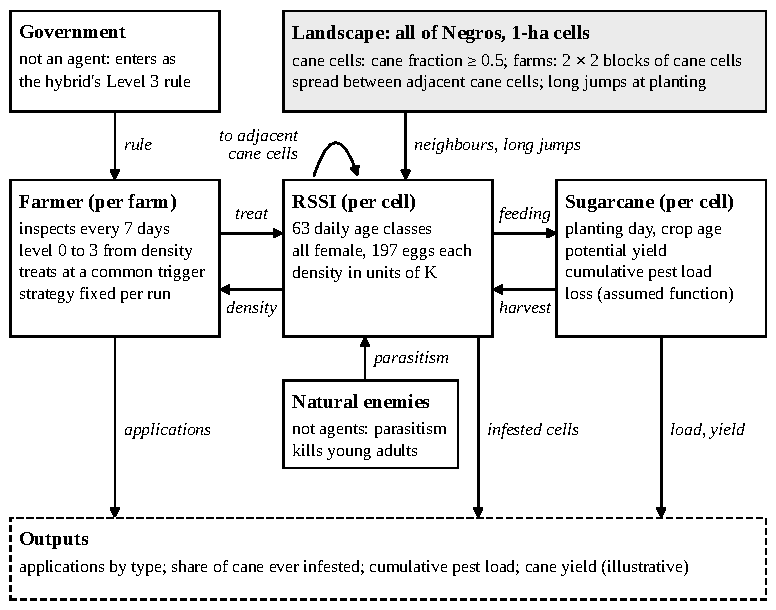
\includegraphics[width=\columnwidth]{figures/fig-conceptual}
\caption{Conceptual model. Pest, crop, and farmer are agents or cell states. Natural enemies and government enter as rules. Climate is held out.}
\label{fig:concept}
\end{figure}

\subsection{Landscape and Data}

The landscape covers all of Negros at 1-ha resolution: 1,327 by 2,224 cells in 57 cities and municipalities \cite{OCHA2025}. Each cell carries the share of its 10-m pixels mapped as sugarcane in a global map for 2019--2022 \cite{DiTommaso2024}, and a cell with at least half its area mapped as cane is a cane cell. This gives 356,869 cane cells (Fig.~\ref{fig:land}). The map predates the outbreak, and its cane area is 1.47 times the area SRA reports as planted in 2025--2026 \cite{SRA2026FOI}. Farms are 2 by 2 blocks of cane cells, an assumption, since no farm-boundary data were found. Roads from OpenStreetMap \cite{OSM2026} are loaded but have no effect at baseline. Window A, the cane of Cadiz City, Manapla, and the City of Victorias (32,335 cane cells, 10,611 farms), is used for runs that need many replicates.

\begin{figure}[t]
\centering
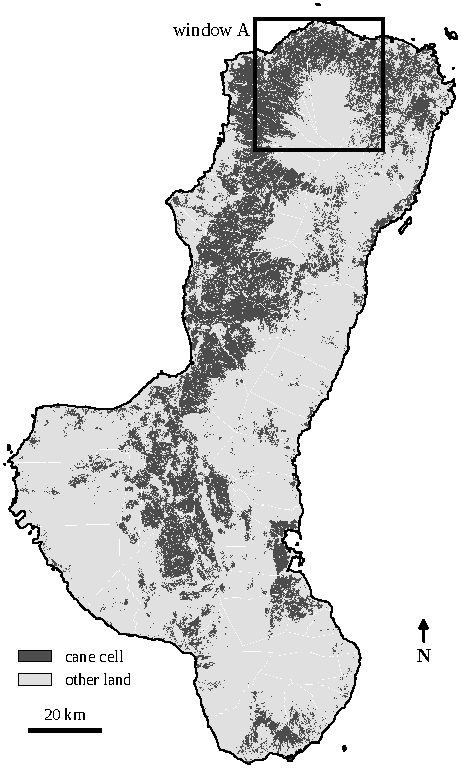
\includegraphics[width=0.62\columnwidth]{figures/fig-landscape}
\caption{Model landscape: cane cells (dark) from the 2019--2022 sugarcane map \cite{DiTommaso2024}, municipal boundaries \cite{OCHA2025}, and window A (box).}
\label{fig:land}
\end{figure}

\subsection{Pest, Spread, and Damage}

One tick is one day. The pest in each cane cell is held as a density in 63 daily age classes, in units of the cell's carrying capacity $K$. Stage durations are fixed inside the Philippine laboratory ranges: egg 2 days, instars of 6, 6, and 5 days, and adult stages of 13, 17, and 14 days \cite{Guerrero2026}. Recruitment is limited by a density-dependent term and by a lumped settlement survival, which has no field estimate. Parasitism removes young adults at a rate set from Luzon observations \cite{Guerrero2024}. Spread is assumed, because no measured rate was found. A planted cell receives crawlers with probability $1-\exp(-\beta P)$, where $P$ is the summed density of its infested cane neighbours, the form used in individual-level models of spatial disease spread \cite{Deardon2010}, and long jumps at planting stand for infested planting material. A wind bias on neighbour spread, with direction from the nearest official normals \cite{PAGASAnd}, is off at baseline. Loss is linear in cumulative pest load. No Philippine study has measured RSSI yield loss \cite{Guerrero2024}, so cane yield is illustrative, and pest load and the share of cane ever infested are the primary outputs.

\subsection{Farmers and Control}

Every 7 days a farmer reads the mean density over its planted cells and assigns a level. The provincial task force defines Levels 1 to 3 as 1 to 5, 6 to 10, and more than 10 insects per leaf \cite{PGNO2026}. No source gives $K$ in insects per leaf, so the conversion assumes 100 insects per leaf at capacity, which gives thresholds of 0.01, 0.06, and 0.11\,$K$. Farmers treat at Level 1 with at least 14 days between treatments, and the same trigger applies to every strategy. A treatment acts on nymphs and adults for 14 days. The chemical kill is the median of six compounds on first application, 74.3\% on nymphs and 54.9\% on adults \cite{SRAnd}. The fungus kills 0.9 times as much, bounded by field and laboratory comparisons \cite{Sallam2021,Buletin2026}. The hybrid uses the fungus at Levels 1 and 2 and a chemical at Level 3, following a report that fungi target Levels 1 and 2 while local governments lead on Level 3 \cite{Gomez2026}; that the Level 3 agent is chemical is an inference. Chemical efficacy halves after a set number of applications on a farm. A test setting applies the same rule to the fungus. Neither represents resistance biology.

\subsection{Initial Conditions and Runs}

The landscape is free of the pest until day 233, 22 May 2025, counted from 1 October 2024. On that day 87 planted cells are seeded at 0.05\,$K$ in the 11 local government units reported as affected four days later \cite{Guadalquiver2025}, split equally because no area by unit was published. Window A holds three of these units, so its 87 cells are 29 per unit. Runs last 1,095 days after seeding. Code checks on the model before the seeded start was added matched the laboratory life table and a pest-free crop baseline.

The island comparison runs six configurations: no control, chemical control with no decline and with efficacy halving every 20 and every 10 applications, biological, and hybrid. Window A repeats the comparison and carries a one-at-a-time sensitivity screen of nine unsourced assumptions at a low and a high value (18 cases plus a baseline, after \cite{Alves2026}), a wind-direction check, a damage-form check, chemical decline at 40, 80, and 160 applications, a hybrid test, and a fungal-decline test. In all, 160 runs were made with GAMA 2026.11.0 in headless mode, one simulation per process. Configurations have two runs, three for island no control, and sensitivity cells have one. Run-to-run noise was pooled over 20 window A pairs. Two-run means are read as different only when their ratio exceeds a two-standard-error band of 1.07 to 1.17, and single runs of the biological and hybrid strategies tie within 1.25.

\subsection{Hindcast}

The model cannot be calibrated, since no infestation series by level exists: SRA mapping is ongoing \cite{SRA2026FOI}, and the provincial survey is one dated snapshot \cite{PGNO2026}. Instead it is read on day 731, 2 October 2026, against the SRA validated area \cite{SRA2026FOI}, for the hybrid and for no control. No-control runs with higher transmission or long-jump rates show what spread would reach that area. The area ever infested by municipality is compared with the SRA figures by Spearman rank correlation, and the split of infested farms across Levels 1 to 3 with the provincial survey \cite{PGNO2026}.

\section{Results and Discussion}

\subsection{Strategy Comparison}

Table~\ref{tab:main} gives the comparison. On window A, no control gave 10.8 million K-days, with 96.5\% of cane cells ever infested. Every control strategy cut the load by at least 82\%. Chemical control without decline gave the lowest load, 0.69 times the pooled biological and hybrid mean of 43,258 K-days (14 runs). Biological and hybrid control were indistinguishable: the hybrid applied no chemical at baseline, and its pooled mean was 1.02 times the biological mean. Chemical control with efficacy halving every 20 and every 10 applications was 17.4 and 44.4 times the biological and hybrid pool. The island runs gave the same order. They are not comparable with window A in size, because the island seed is spread over 11 units and the island has about 11 times as much cane.

\begin{table}[t]
\caption{Cumulative Pest Load (K-days, Mean of Runs) and Share of Cane Cells Ever Infested, 1,095 Days After Seeding}
\label{tab:main}
\centering
\footnotesize
\begin{tabular}{@{}lrrrr@{}}
\toprule
 & \multicolumn{2}{c}{Window A} & \multicolumn{2}{c}{Island} \\
Strategy & Load & Ever & Load & Ever \\
\midrule
Chemical, no decline & 30,013 & 0.19 & 43,950 & 0.027 \\
Hybrid, decline 20 & 42,789 & 0.26 & 63,067 & 0.038 \\
Biological & 44,123 & 0.26 & 60,394 & 0.036 \\
Chemical, decline 20 & 754,011 & 0.34 & 982,778 & 0.051 \\
Chemical, decline 10 & 1,919,710 & 0.49 & 2,539,217 & 0.082 \\
None & 10,763,962 & 0.97 & 33,213,080 & 0.64 \\
\bottomrule
\end{tabular}
\\[2pt]
\parbox{\columnwidth}{\footnotesize Two runs per configuration, three for island no control. Decline $n$: chemical efficacy halves every $n$ applications per farm. The hybrid applied no chemical.}
\end{table}

\subsection{Efficacy Decline}

Fig.~\ref{fig:decline} shows chemical control across decline rates. With efficacy halving every 160 or 80 applications per farm, chemical control stayed within or below the biological and hybrid range (0.79 and 0.90 times the pool). At 40 applications it was 3.9 times worse. Chemical control therefore matches biological control only if its efficacy halves no faster than about every 80 applications. This advantage of the fungus follows from the assumption that its efficacy does not decline. When the fungus halved every 20 applications, biological control gave 1,205,918 K-days, 1.60 times chemical control at the same rate, and the hybrid gave the lowest load, 0.32 times biological and 0.51 times chemical. At 80 applications, biological control was 1.95 times chemical, and the hybrid tied with biological (ratio 0.89). This is likely because the hybrid counts the two agents' applications separately, so switching spreads the decline across them.

\begin{figure}[t]
\centering
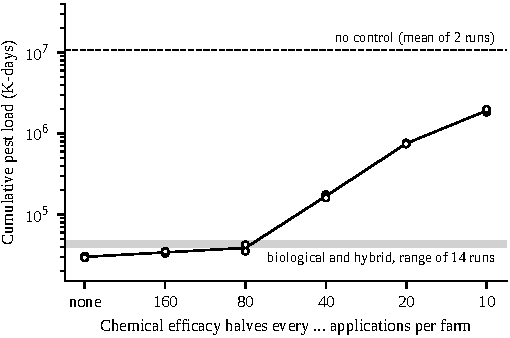
\includegraphics[width=\columnwidth]{figures/fig-decline}
\caption{Chemical control on window A by efficacy-decline rate. Circles are single runs, the line joins means. The band is the range of 14 biological and hybrid runs at baseline. Fungal efficacy does not decline.}
\label{fig:decline}
\end{figure}

The hybrid differs from biological control only where farms reach Level 3. Treating at Level 1 every 14 days kept them below it. In the screen, the hybrid applied chemicals only where treatment was delayed: a trigger at Level 2 or 3, or re-treatment every 28 days. Rerun with non-declining chemical control, these settings gave a tie when treating only at Level 3 (ratios 0.89 to 1.04), and an ordering of chemical (262,998 K-days), hybrid (693,075), and biological (1,119,909) when re-treating every 28 days. While fungal efficacy holds, the hybrid adds nothing. It helps when both agents lose efficacy quickly.

\subsection{Sensitivity}

The baseline ranking, biological and hybrid tied, then chemical with decline 20, then no control, held in 15 of 18 cases (Table~\ref{tab:oat}). No control was last in all 18. When treatment waited for Level 3 or was repeated every 28 days, biological control ranked first. When settlement survival was 0.01, chemical control ranked first, but the outbreak was about 26 times smaller, so this ranking is less certain. The response rules mattered more than any biological parameter: for biological control, waiting for Level 2 raised the load 16.6 times and waiting for Level 3, 33 times. Wind bias, wind direction, long-jump rate, and the fungus-to-chemical ratio moved loads by less than 1.5 times. Runs with wind from the south-west gave 0.96 to 1.11 times the load of runs with wind from the north-east, inside the noise bands.

\begin{table}[t]
\caption{One-at-a-Time Screen on Window A: Largest Change in Load (log$_{10}$ Ratio to Baseline) Over the Four Strategies}
\label{tab:oat}
\centering
\footnotesize
\begin{tabular}{@{}lll@{}}
\toprule
Assumption & Low, high & Change \\
\midrule
Settlement survival & 0.01, 0.10 & 1.96 \\
Trigger level & 2, 3 & 1.81 \\
Re-treatment interval & 7, 28 d & 1.49 \\
Parasitism & 0, 0.668 & 1.16 \\
Neighbour transmission & $\times$0.25, $\times$4 & 0.86 \\
Level thresholds & $\times$0.5, $\times$2 & 0.59 \\
Long-jump probability & 0, 0.2 & 0.17 \\
Fungus-to-chemical ratio & 0.8, 1.0 & 0.17 \\
Wind bias & 0.5, 1.0 & 0.06 \\
\bottomrule
\end{tabular}
\\[2pt]
\parbox{\columnwidth}{\footnotesize One run per cell. The ranking changed for settlement survival 0.01, trigger at Level 3, and re-treatment every 28 days.}
\end{table}

\subsection{Hindcast}

Table~\ref{tab:hind} compares the model with the SRA record. At baseline the model spread too slowly: even without control it reached 0.30 of the validated area. A threefold transmission rate brought no control to 0.98 of it. That rate is one parameter tuned to one number with control ignored, and it was not used in the comparison. It also fell short earlier in the outbreak: 2,861 ha against 4,923 ha recorded for Negros Island on 11 September 2025 \cite{MojicaSevilla2025}. No run matched which municipalities were worst affected (rank correlations of $-0.29$ to 0.22 outside the seeded units). In the hybrid run all infested farms stayed at Level 1, while the survey found 53\%, 31\%, and 16\% of infested farmlots at Levels 1 to 3 \cite{PGNO2026}. Real response is slower and less complete than the model's weekly, error-free trigger: only about 53\% of the validated area had been treated by 2 October 2026 \cite{SRA2026FOI}.

\begin{table}[t]
\caption{Hindcast, 2 October 2026: Model Cane Area Ever Infested Against 72,103 ha Validated by SRA}
\label{tab:hind}
\centering
\footnotesize
\begin{tabular}{@{}lrrr@{}}
\toprule
Run & Area (ha) & Ratio & $\rho$ \\
\midrule
Hybrid, baseline & 2,908 & 0.04 & 0.10 \\
None, baseline & 21,275 & 0.30 & $-0.29$ \\
None, long jump 0.2 & 44,072 & 0.61 & 0.22 \\
None, transmission $\times$2.5 & 58,136 & 0.81 & $-0.09$ \\
None, transmission $\times$3 & 70,430 & 0.98 & $-0.18$ \\
None, transmission $\times$4 & 105,535 & 1.46 & $-0.04$ \\
\bottomrule
\end{tabular}
\\[2pt]
\parbox{\columnwidth}{\footnotesize Hybrid: mean of two runs. Others: one run. $\rho$: Spearman correlation with the SRA share by municipality, 45 unseeded units.}
\end{table}

\subsection{Limitations}

Spread, settlement survival, and seed size are uncalibrated, and the hindcast shows baseline spread is too slow. Farmers respond more promptly than observed \cite{SRA2026FOI,PGNO2026}. The fungus's efficacy and its persistence are assumed. Without a dose-response there are no yield or income results. Delivery by truck or backpack sprayer, which depends on field access \cite{PGNO2026}, is not modelled. Configurations have two runs and the screen one, so differences are read only against pooled noise bands, and the random seed was not logged, so single runs cannot be reproduced exactly. Sensitivity was screened on window A only. The land-cover map dates from 2019--2022 and overstates planted area \cite{DiTommaso2024,SRA2026FOI}.

\section{Conclusion}

The model compares RSSI strategies on the Negros cane landscape with every unmeasured input exposed. Within its assumptions, any control beats none, acting early matters more than which agent is used, and the ranking of chemical against biological control turns on two unmeasured quantities: how fast chemical efficacy declines and whether fungal efficacy holds. Data on repeated-application efficacy of both agents, the spread rate between fields, and the timing of real treatment would most change the answer.

\bibliographystyle{IEEEtran}
\bibliography{ieee}

\end{document}
